\documentclass[a4paper, 14pt]{article}				% general format

\usepackage[utf8]{inputenc}					% accept different input encodings
\usepackage[russian]{babel}					% multilingual support (T2A)
\usepackage{graphicx}
\usepackage{float}
\usepackage{amsmath}

\author{Певцов Игорь, гр.53501/3}
\title{Отчет по лабораторным работам 1-3:\\"\LaTeX{}, Git, GPG"\\ по дисциплине\\"Методы и средства защиты информации"}

\begin{document}
\maketitle

\newpage
\tableofcontents{}

\newpage

\section{Cистема верстки \TeX{} и расширения \LaTeX{}}

\subsection{Цель работы}
Изучение принципов верстки \TeX{}, создание первого отчёта.
\subsection{Ход работы}
Файл .tex представляет из себя обычный текстовый файл содержащий макрокоманды текстовой разметки. Создать файл можно в любом текстовом редакторе, сохранив его с расширением .tex (Рис. 1).

\begin{figure}[h!]
\centering
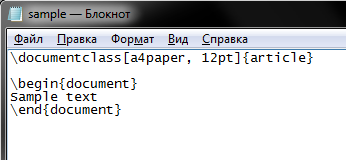
\includegraphics[width=0.5\textwidth]{fig1}
\caption{Простейший ТеХ документ.}
\end{figure}

\subsubsection{Компиляция в командной строке}
Компиляция исходного текста может производиться при помощи командной строки. После компиляции командой LATEX выходной файл имеет формат DVI(DeVice Independent) - аппаратно независимый формат файла, содержащий двоичные данные и не предназначенный для чтения человеком (Рис. 2). 

\begin{figure}[h!]
\centering
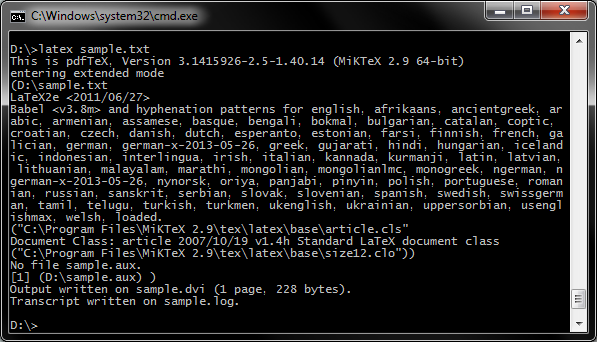
\includegraphics[width=0.5\textwidth]{fig2}
\caption{Компиляция в DVI-файл.}
\end{figure}

Для перевода файла в читабельный вид(PDF-файл) необходимо выполнить команду PDFLATEX (Рис. 3).

\begin{figure}[h!]
\centering
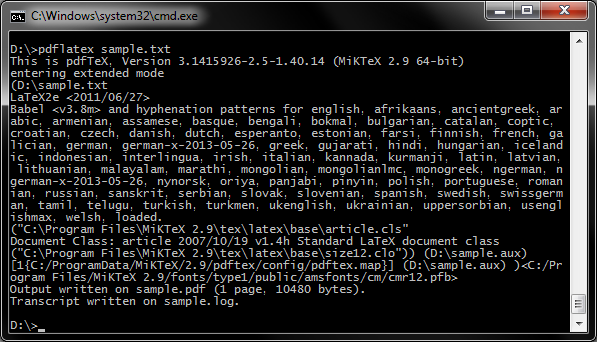
\includegraphics[width=0.5\textwidth]{fig3}
\caption{Получение PDF файла.}
\end{figure}

\subsubsection{Оболочка TeXworks}
Для выполнения работы был использован дистрибутив MiKTeX 2.9 для Windows. Данный дистрибутив включает в себя редактор TeXworks (Рис. 4) с интуитивно понятным интерфейсом, а также интегрированный и отдельный менеджеры пакетов. Редактор позволяет выбрать инструменты верстки в выпадающем меню и сразу же начать верстку нажатием кнопки. Также, в редакторе сразу же доступно окно просмотра PDF-файлов (справа на Рис. 4). Редакотр поддерживает добавление сценариев для расширения списка доступных функций редактора. 
\begin{figure}[h!]
\centering
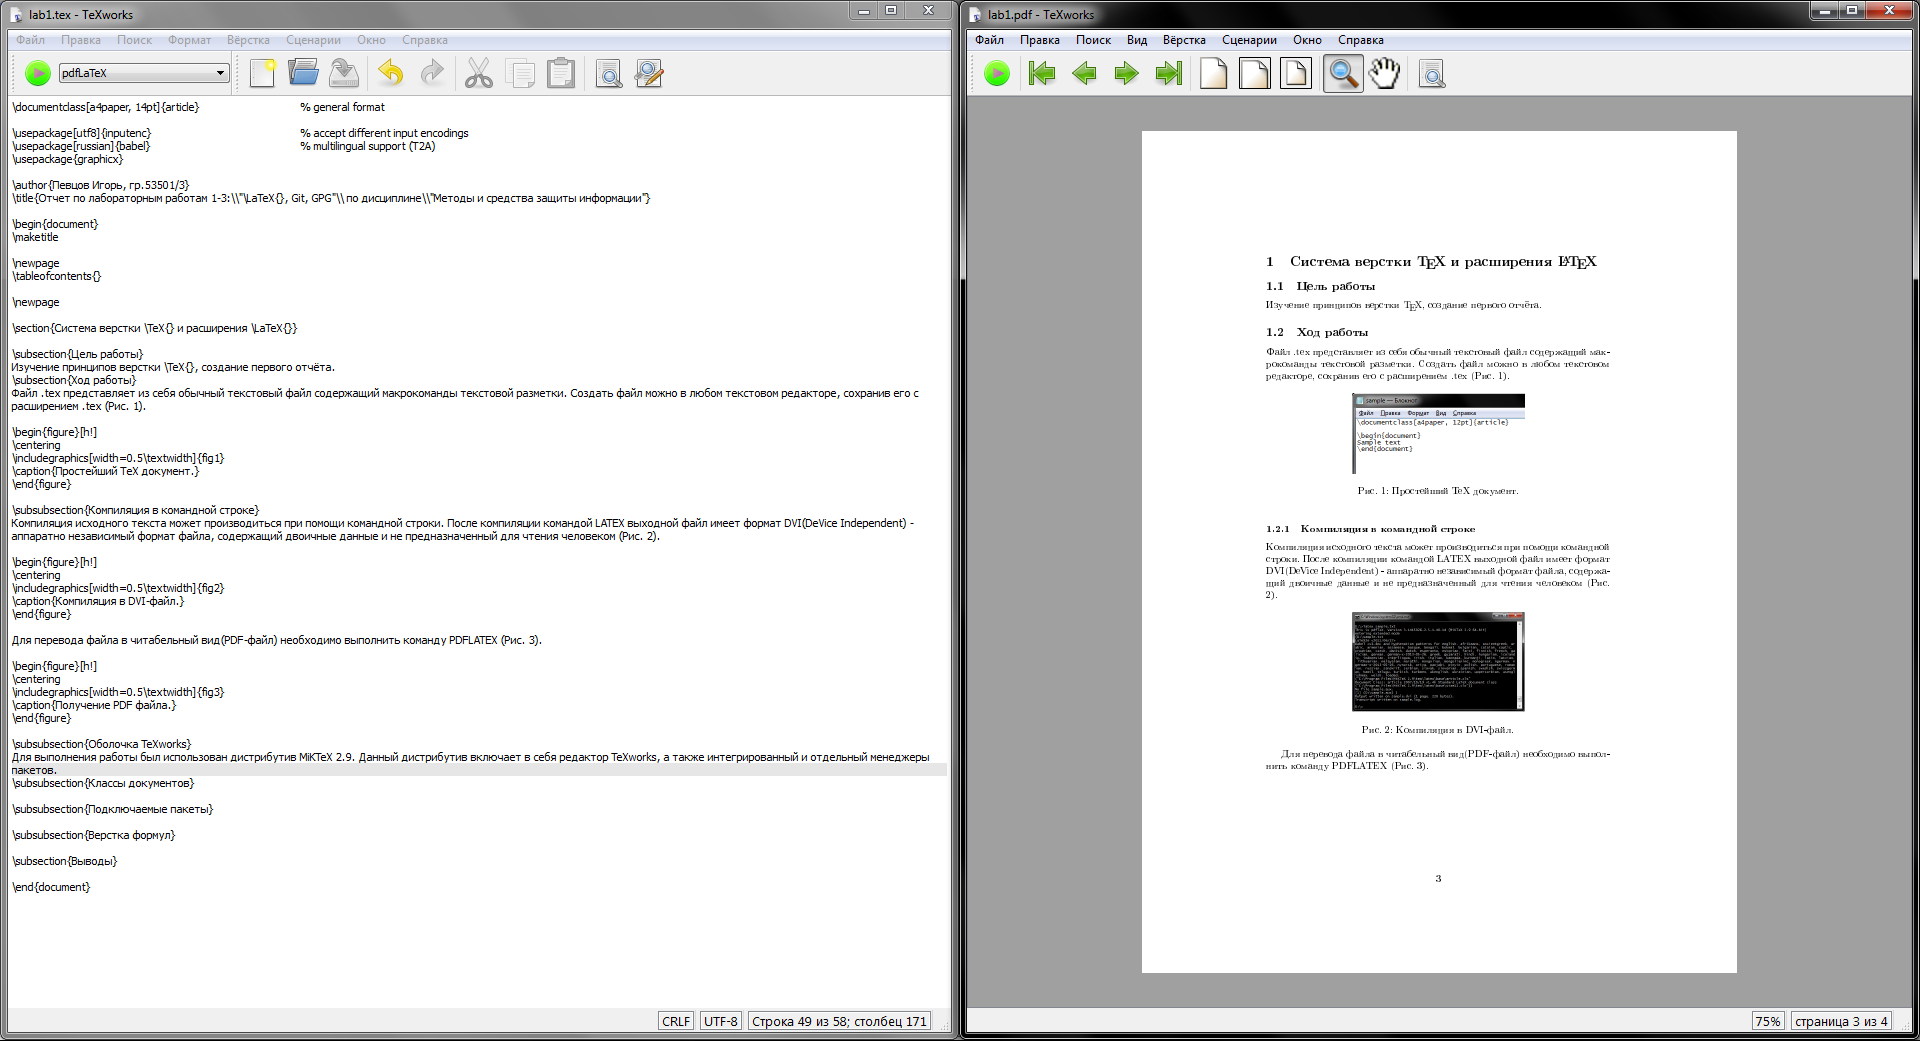
\includegraphics[width=\textwidth]{fig4}
\caption{Интерфейс редактора TeXworks.}
\end{figure}

\subsubsection{Создание титульного листа, нескольких разделов, списка, несложной формулы}
Создание простейшего титульного листа включает в себя задаваемые в преамбуле заголовок и имя автора. Для наполнения титульного листа используются команды:

\begin{verbatim}
	\author{Певцов Игорь, гр.53501/3}
	\title{Отчет по лабораторным работам 1-3:\\"\LaTeX{}, Git, GPG"\\
	 по дисциплине\\"Методы и средства защиты информации"}
\end{verbatim}

Непосредственно создание заголовка:
\begin{verbatim}
	\maketitle
\end{verbatim}

\begin{figure}[h!]
\centering

\includegraphics[width=0.6\textwidth]{fig5}
\caption{Титульный лист.}
\end{figure}

Создание разделов:
\begin{verbatim}
	\part[1]{Раздел 1}
	\part[2]{Раздел 2}
	\part[3]{Раздел 3}
\end{verbatim}

\begin{figure}[h!]
\centering
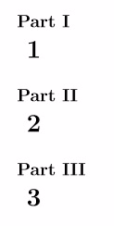
\includegraphics[width=0.1\textwidth]{fig6}
\caption{Разделы.}
\end{figure}

Создание списков (ненумерованых):
\begin{verbatim}
	\begin{itemize}
		\item{one}
		\item{two}
		\item{three}
	\end{itemize}
\end{verbatim}

Получившийся список:
\begin{itemize}
	\item{one}
	\item{two}
	\item{three}
\end{itemize}

Запись формул. 
\begin{verbatim}
	$f(x,y)= 3x^3 + 15y^2 + 10$
\end{verbatim}

Получившаяся формула:
$f(x,y)= 3x^3 + 15y^2 + 10$

Более сложные формулы набираются с использованием 
\begin{verbatim}
	\begin{equation}
		formula
	\end equation
\end{verbatim}

\subsubsection{Классы документов, подключаемые пакеты}
Каждый файл в \LaTeX{} начинается с команды documentclass[...]{...}, в фигурных скобках которой задаются параметры оформления стиля документа, а в квадратных — список классовых опций.
Всего в \LaTeX{} 5 основных классов документов:
\begin{itemize}
\item {article для статей}
\item {report для книг и статей}
\item {book для книг}
\item {proc для докладов}
\item {letter для оформления деловых писем} . 
\end{itemize} 
Помимо основных, есть ещё множество дополнительных.

В \LaTeX{} помимо стандартных настроек существует возможность подключения сторонних пакетов со специфическими настройками. Такие пакеты расширений подключаются в шапке документа.
\begin{verbatim}
	usepackage{listings} % предоставляет возможности цитирования 
кода в тексте с сохранением исходного форматирования.
\end{verbatim}
\subsubsection{Верстка сложных формул}
Сложные формулы, на которые надо будет ставить ссылки в тексте, можно набирать, используя класс equation. Все ссылки подсчитываются автоматически, надо лишь сослаться на какую-либо ссылку при помощи команды ref.
\begin{equation}
  L' = {L}{\sqrt{1-\frac{v^2}{c^2}}}
 \end{equation}
\subsection{Выводы}
\LaTeX{} очень удобен при наборе сложных документов, имеющих множество формул, разделов и пр. \LaTeX{} позволяет сконцентрироваться на изменении содержания документа и переложить все форматирование на систему верстки. Пакет позволяет автоматизировать многие задачи набора текста и подготовки статей, включая набор текста на нескольких языках, нумерацию разделов и формул, перекрёстные ссылки, размещение иллюстраций и таблиц на странице, ведение библиографии и др. Кроме базового набора существует множество пакетов расширения \LaTeX{}. Готовя свой документ, автор указывает логическую структуру текста (разбивая его на главы, разделы, таблицы, изображения), а \LaTeX{} решает вопросы его отображения. Так содержание отделяется от оформления. Оформление при этом или определяется заранее (стандартное), или разрабатывается для конкретного документа.

\newpage
\section{Система контроля версий Git}
\subsection{Цель работы}
Изучить систему контроля версий Git, освоить основные приемы работы с ней.
\subsection{Ход работы}
\subsubsection{Получение содержимого репозитория}
Содержимое репозитория получается простой консольной командой 
\begin{verbatim}
	git clone https://github.com/magniii/InfoSecCourse2015.git
\end{verbatim}

\subsubsection{Добавление новой папки и файла под контроль версий}
Добавление папок и файлов производится командой add с различными вариациями аргументов. Аргумент --all указывает на то, что Git должен добавить всю текущую директорию под контроль версий
\begin{verbatim}
	mkdir testdir
	cd testdir
	echo abcd >> tmp
	git add --all
\end{verbatim}

\subsubsection{Фиксация изменений в локальном репозитории}
Изменения в локальном репозитории фиксируются командой commit
\begin{verbatim}
	git commit -a -m "pew"
\end{verbatim}

\subsubsection{Просмотр различий после внесения изменений в файл}
Просмотр различий выполняется командой diff
\begin{verbatim}
	echo 123 >> tmp
	git diff master:./tmp ./tmp
\end{verbatim}

\subsubsection{Отмена локальных изменений}
Сброс выполняется командой reset. Команда checkout возвращает репозиторий к указанному состоянию.
\begin{verbatim}
	git reset HEAD ./tmp
	git checkout ./tmp
\end{verbatim}

\subsubsection{Просмотр различий после внесения изменений в файл}
\begin{verbatim}
	echo qwerty >> tmp
	git diff master:./tmp ./tmp
\end{verbatim}

\subsubsection{Фиксация изменений в локальном и центральном репозиториях}
\begin{verbatim}
	git commit -a -m "pew2"
	git push
\end{verbatim}

\subsubsection{Получение изменений из центрального репозитория}
\begin{verbatim}
	git pull
\end{verbatim}

\subsubsection{Поэксперементировать с ветками}
\begin{verbatim}
	git checkout -b tmpbranch
	git commit -a -m "pew3"
	git push
	git checkout master
	git merge tmpbranch
	git branch -D tmpbranch
\end{verbatim}

\subsection{Выводы}
Система контроля версий Git ориентирована на работу с изменениями, а не с файлами. Преимуществами системы перед другими распределенными системами контроля версий является высокая производительность, развитые средства интеграции с другими VCS и продуманная система команд.Из недостатков можно отметить отсутствие сквозной нумерации коммитов, привязанность к ANSI-символам и применение хэшей SHA1 для идентификации ревизий.

\newpage
\section{GPG}
\subsection{Цель работы}
Научиться создавать сертификаты, шифровать файлы и ставить ЭЦП.
\subsection{Ход работы}
\subsubsection{Создание ключевой пары OpenPGP}
\begin{figure}[h!]
\centering
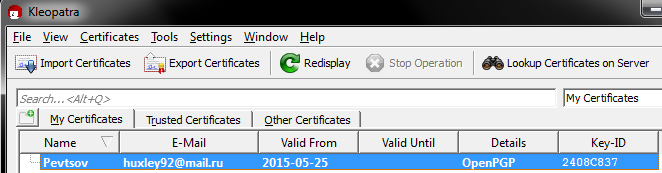
\includegraphics[width=\textwidth]{fig8}
\caption{Ключи созданы.}
\end{figure}

\subsubsection{Экспорт ключевой пары}
\begin{figure}[h!]
\centering
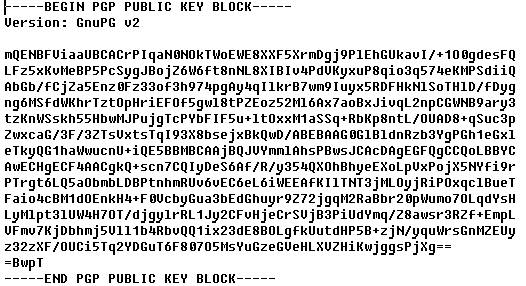
\includegraphics[width=0.8\textwidth]{fig9}
\caption{Ключи экспортированы.}
\end{figure}

\subsubsection{Установка ЭЦП на файл}
\begin{figure}[h!]
\centering
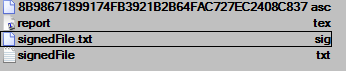
\includegraphics[width=0.7\textwidth]{fig10}
\caption{Файл подписан ЭЦП.}
\end{figure}

\subsubsection{Получение чужого сертификата}
\begin{figure}[h!]
\centering
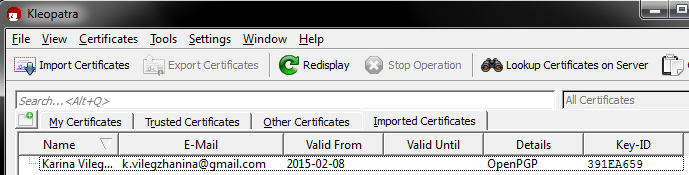
\includegraphics[width=\textwidth]{fig11}
\caption{Чужой сертификат (karina.asc) подписан.}
\end{figure}

\subsubsection{Проверка чужой подписи импортированным сертификатом}
\begin{figure}[h!]
\centering
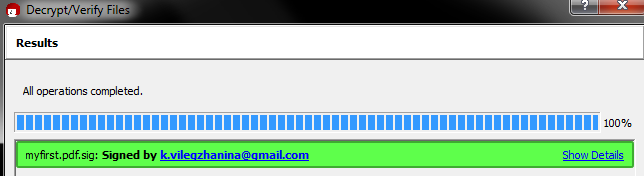
\includegraphics[width=\textwidth]{fig12}
\caption{Подлинность файла myfirst.pdf.sig подтверждена.}
\end{figure}

\subsubsection{Работа с командной строкой}
Создание ключа осуществляется командой:
\begin{verbatim}
	gpg --gen-key
\end{verbatim}

\begin{figure}[h!]
\centering
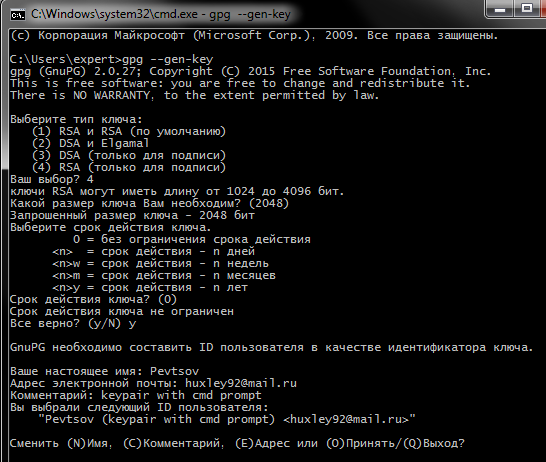
\includegraphics[width=\textwidth]{fig13}
\caption{Создание ключа через консоль.}
\end{figure}
Просмотреть список ключей можно используя команду list
\begin{verbatim}
	gpg --list-keys
\end{verbatim}

\begin{figure}[h!]
\centering
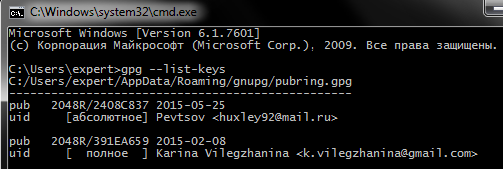
\includegraphics[width=\textwidth]{fig14}
\caption{Просмотр списка ключей.}
\end{figure}

Для импорта ключей используется команда
\begin{verbatim}
	gpg --import importable.asc
\end{verbatim}
Для экспорта применяется команда
\begin{verbatim}
	gpg --armor --output exportable.asc --export exporter@mail.ru
\end{verbatim}

\subsection{Выводы}
GPG позволяет выполнять операции шифрования и цифровой подписи сообщений, файлов и другой информации, представленной в электронном виде, в том числе прозрачное шифрование данных на запоминающих устройствах, например, на жёстком диске. GPG включает в себя внутреннюю схему проверки сертификатов, названную web of trust. GPG поддерживает аутентификацию и проверку целостности посредством цифровой подписи. По умолчанию она используется совместно с шифрованием, но также может быть применена и к открытому тексту. Отправитель использует GPG для создания подписи алгоритмом RSA или DSA.
\end{document}